\section{Data Sources}\label{sec:source}

Previous surveys such as  \cite{Tao2005, Zhang2014, Poria2017, Garcia-Garcia2017} put forward that in multimodal affective computing with different data sources should be applied with different modelling methods. \cite{Poria2017} also give the argument 90\% literature consider visual, audio and text information as multimodal affect analysis by their extensive literature review.

In this section, we discusses the commonly exists data sources in smartphone, and prepare for the modelling method in the next section. Figure \ref{fig:source} illustrates the data flow from sensors to user emotion state.

\begin{figure}
    \centering
    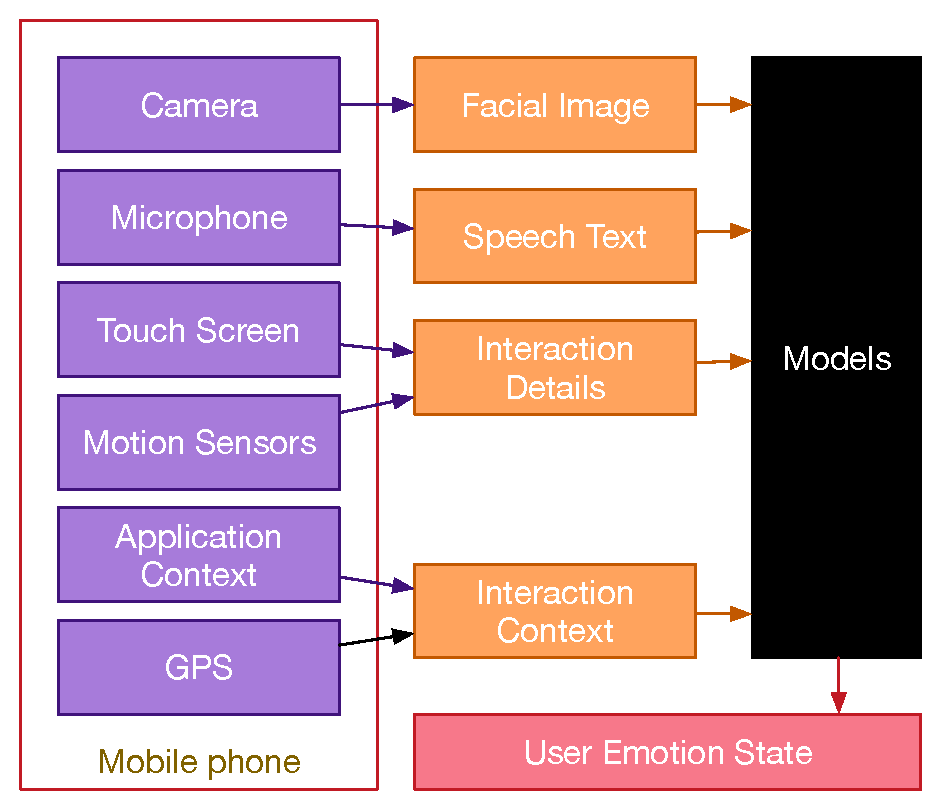
\includegraphics[width=0.5\textwidth]{source}
    \caption{Data sources can be used in emotion inferring which provided by the most of commercial mobile phone devices.}
    \label{fig:source}
\end{figure}

\subsection{Camera}\label{subsec:vision}
We emphasis vision sensors in the first place since face and facial expressions are undoubtedly one of the most important nonverbal channels used by the human being to convey internal emotion. This part mainly discusses vision sensors, which includes RGB camera and depth camera, and illustrates how vision sensor can be used for affective emotion inferring.

Pure RGB cameras has been widely used in commercial smartphone as image sensor. 
For the camera with depth informations on mobile (recently introduced TrueDepth Camera (see Figure \ref{fig:ipx}) in iPhone X \footnote{\url{https://www.apple.com/iphone-x/\#truedepth-camera}}) combines infrared camera, flood illuminator, proximity sensor, ambient light sensor, front facing camera and dot projector to provide depth images of facial information of a user.

\begin{figure}
    \centering
    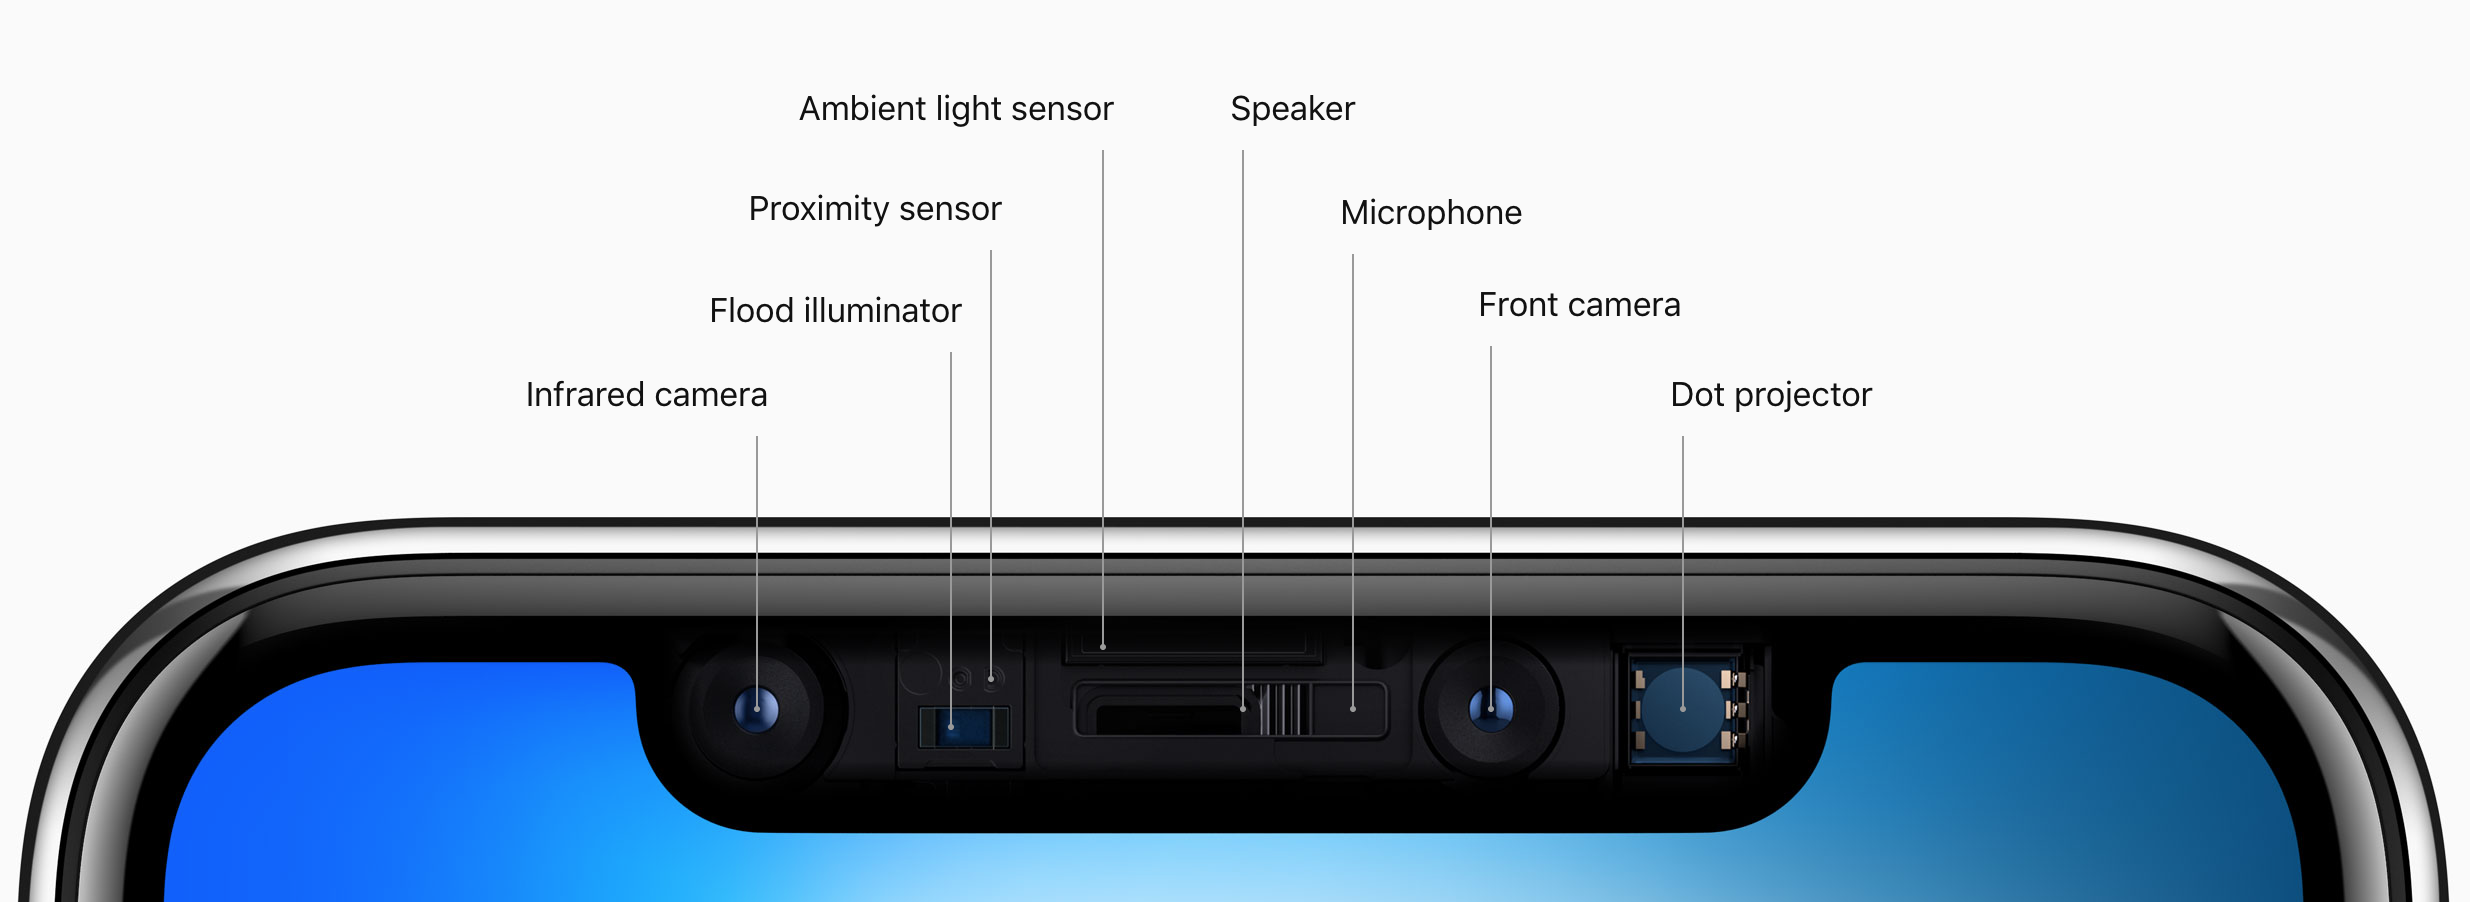
\includegraphics[width=0.5\textwidth]{ipx}
    \caption{TrueDepth Camera in iPhone X.}
    \label{fig:ipx}
\end{figure}

\subsection{Microphone}\label{subsec:audio}
Audio sensor usually refers to built-in microphones, it collects voice information from current environments, which can infers user emotions based on their speech contents.

Inferring emotions from user speech can split as two part of inferring task. The first part is recognize the speech text from user, then understanding or inferring from text.

% TODO add more

\subsection{Touch Screen}\label{subsec:touch}

Human emotions can be epxressed in different ways, emotional communication has focused predominantly on the facial and vocal channels but has ignored the tactile channel\cite{hertenstein2009communication}, which investigated the possible expressions of user emotion in detail while they using mobile devices with touch screen.

Capacitive touch screen provides touch position, touch pressure, touch angle through time. Among the subsequent researches\cite{Gao2012, Shah2015, Mottelson2016, bhattacharya2017predictive}, researchers explored yeild results that human emotions can be inferred by capacitive touch channel in a specific application context based on these features, whose are the existed typical research on emotion inferring only with touch screen interface.

Interestingly, 3D touch screen was introduced in commercial devices few years ago, some of researches investigated the haptic  \cite{Eid2016} 
\cite{Mazzoni2016, Lentini2017} shows a system with haptic touch response essentially can express and influence user emotions. and \cite{Bhattacharya2017} concludes that haptic-based affect detection remains an understudy topic.

\subsection{Motion Sensors}\label{subsec:motion}

Motion sensors typically combines gyroscope and accelerometer. Accelerometer measures proper acceleration (acceleration it experiences relative to free fall), felt by people or objects, units as $m/s^2$ or $g$ (1g when standing on earth at sea level). Most smartphone accelerometers trade large value range for high precision. Gyroscope can be a very useful tool because it moves in peculiar ways and defy gravity. Gyroscopes have been around for a century, and they are now used everywhere from airplanes, toy helicopters to smartphones. A gyroscope allows a smartphone to measure and maintain orientation. Gyroscopic sensors can monitor and control device positions, orientation, direction, angular motion and rotation. Figure \ref{fig:motion} shows the coordinates information of accelerometer and gyroscopy sensors.

\begin{figure}
    \centering
    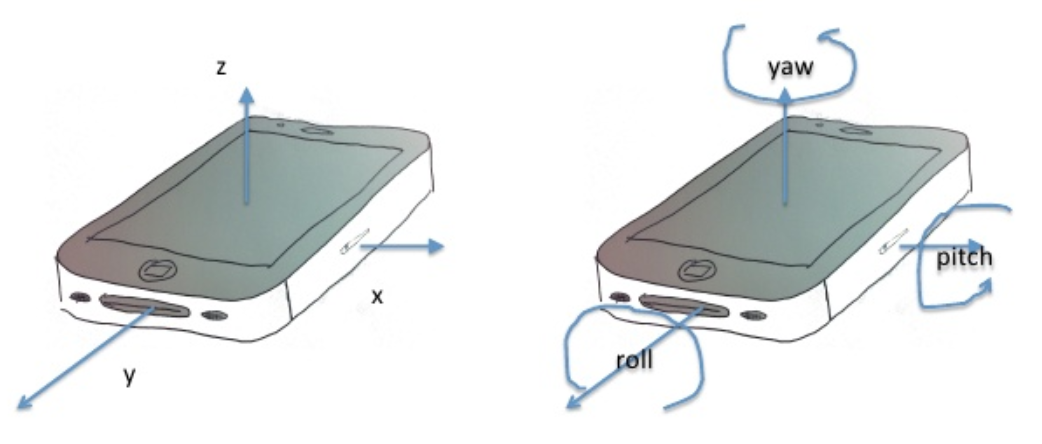
\includegraphics[width=0.5\textwidth]{motion}
    \caption{Coordinates information of Accelerometer (left) and gyroscope (right) as motion sensors in iOS CoreMotion framework.}
    \label{fig:motion}
\end{figure}

\subsection{GPS}\label{subsec:gps}

GPS sensors provides geographical information of a user, it detects the location of the smartphone using 1) GPS; 2) Lateration/Triangulation of cell towers or wifi networks (with database of known locations for towers and networks); 3) Location of associated cell tower or WiFi networks.

However, GPS will not work indoors and can quickly kill battery. Smartphones can try to automatically select best-suited alternative location provider (GPS, cell towers, WiFi), mostly based on desired precision. With the location, we can study the relationship between life patterns and affective states. For example, most people in playground feel happy while most feel sad in cemetery.

Location provides additional information to verify the subjective report from participants of affective studies. It may also help to build a confidence mechanism \cite{tan2013connectivity} for subjective reports. Attaching the location to the subjective report would produce confident weights to measure the significance of col- lected subjective reports. For example, a participant reported that he was happy in cemetery. But, in common sense, people in cemetery would be sad. Thus, we could set a low weight (e.g., 0.2) as a confident value to the report.

\subsection{Application Context}\label{subsec:ui}

As we slightly mentioned in previous section, most of the mobile affective inferring techniques based on touch scree and motion sensors\cite{Gao2012, Shah2015, Mottelson2016, bhattacharya2017predictive} are based on specific application context, for example application user interface. This can be another confidence mechanism for inferring system. Vice versa, the inferring systems are only modelling for a specific context, however this could be a drawback of multimodal emotion inferring since a complete system will integrate more models.